\documentclass[12pt, a4paper]{article}
\usepackage[utf8]{inputenc}
\usepackage[brazilian]{babel}
\usepackage{amsmath}
\usepackage{amsfonts}
\usepackage{amssymb}
\usepackage{verbatim}
\usepackage[T1]{fontenc}
\usepackage{graphicx}
\usepackage[top=2cm, bottom=2cm, left=3cm, right=2cm]{geometry}
\usepackage{makeidx}
\newcounter{prob}
\newcounter{subprob}
\renewcommand{\thesubprob}{\alph{subprob}}

\newcommand{\problem}{\setcounter{subprob}{0} \stepcounter{prob} \par \medskip \noindent \textbf{Problema~\theprob \ }}

\newcommand{\answer}{\par \medskip \noindent \textit{Resposta \ }}

\newcommand{\finalanswer}[1]{
	\begin{center} 
    	{\renewcommand{\arraystretch}{1.5}
		\renewcommand{\tabcolsep}{0.2cm} 
    	\begin{tabular}{|c|} 
    		\hline 
        	$ \displaystyle #1 $  \\ 
        	\hline 
    	\end{tabular}} 
   	\end{center}}

\newcommand{\subproblem}{\stepcounter{subprob} \par \smallskip \noindent \quad \textit{(\thesubprob) \ }}

\newcommand{\subanswer}{\par \smallskip \noindent \quad \textit{Resposta \ }}

\newcommand{\option}{\item[$\square$]}
\newcommand{\thisone}{\item[$\blacksquare$]}

\newenvironment{subitemize}{\begin{itemize}}{\end{itemize}}
\usepackage[tocflat]{tocstyle}
\usetocstyle{standard}



\makeatletter
\renewcommand\tableofcontents{
  \null\hfill\textbf{\Large\contentsname}\hfill\null\par
  \@mkboth{\MakeUppercase\contentsname}{\MakeUppercase\contentsname}
  \@starttoc{toc}
}
\makeatother

\author{COPES - UFS}
\title{Modelo_Relatorio_Parcial}
\date{}
%\Marginsize marginsize { 1 centímetro } {2 } { 4 em em} { 6 pt } 

\begin{document}

\begin{figure}[!h]
    \centering
    
\includegraphics[scale=1.2]{ufs.png}

  \end{figure}
%%--CABEÇALHO--%%

 \begin{center}
 
 \Large UNIVERSIDADE FEDERAL DE SERGIPE
PRÓ-REITORIA DE PÓS-GRADUAÇÃO E PESQUISA
COORDENAÇÃO DE PESQUISA
\vspace{10mm} 

\normalsize PROGRAMA DE INICIAÇÃO CIENTÍFICA VOLUNTÁRIA – PICVOL

\vspace{20mm}

\textbf{\Large CONTROLE ÓPTIMO EM TERAPIAS DE CÂNCER}

\vspace{20mm}
 {\normalsize Área do conhecimento: Matemática\\
Subárea do conhecimento: Equações Diferenciais Parciais\\
Especialidade do conhecimento: Oncologia Matemática\\}
\vspace{20mm}

{\normalsize Relatório Final\\
Período da bolsa: de 08/2017 a 08/2018}
\vspace{10mm}

 {\large Este projeto é desenvolvido de forma voluntária}
\vspace{10mm}

\large{PICVOL}


 \end{center}

 
\newpage

 
 \begin{flushleft}
 
\tableofcontents 


\end{flushleft}
\newpage

\section{ Introdução}

Câncer é o conjunto de mais de 100 doenças, cujo ponto em comum é o crescimento desordenado de células que invadem tecidos e órgãos.\

Nos últimos anos o número de casos tem aumentado e segundo estimativas da Organização Mundial de Saúde o número de novos casos só irão aumentar nos próximos 20 anos. Tornando o câncer a principal causa de morte, superando as doenças cardiovasculares e cerebrovasculares. \

Um dos métodos utilizados para combater o câncer é a radioterapia. Consiste em aplicar feixes de radiações ionizantes, com o objetivo de, através de uma alteração no DNA, impedir a divisão das  tumorais.\

Com o intuito de estudar a dinâmica do crescimento de tumores, junto com o tratamento de radioterapia, fomos introduzidos a temas como o Cálculo Variacional e a Teoria de Controle. Além da introdução de conteúdos novos, foi possível ver na prática, aplicações de conteúdos apresentados em disciplinas da graduação, como o Cálculo e Álgebra Linear. Aumentando assim a compreensão e o interesse por essas disciplinas.\

Continua...

\newpage

\section{Objetivos}
Introduzir o tema da dinâmica do crescimento de tumores para que fosse possível para o aluno entender as publicações atuais, na área. Para que seja possível dar os primeiros passos na pesquisa em direção a publicações próprias.

\newpage

\section{Revisão da Literatura}

Faremos aqui um breve relato do que foi estudado durante a iniciação científica, sendo que os temas, devido a sua complexidade, foram expostos pelo orientador e  co-orientador, cabendo ao orientando aplicá-los na segunda fase no contexto de otimização de terapias de câncer. Nossas principais referências foram os livros (Colocar referencias).
Começamos sendo apresentados a alguns problemas clássicos, para motivar o estudo do cálculo de variações, como por exemplo o problema da braquistócrona.

\begin{itemize}
\item O problema da braquistócrona
\end{itemize}

O problema da braquistócrona, proposto por Johann Bernnoulli em 1696, consiste em encontrar uma curva que uma partícula deve descrever ao se deslocar de um ponto A até um ponto B situados em um mesmo plano vertical, no menor tempo possível, apenas sob a ação da gravidade. Neste caso o ponto A é suposto estar acima do ponto B, mas não na mesma vertical. Se A e B estiverem na mesma vertical, a solução é uma reta.


\begin{center}
\begin{figure}[!h]
	\centering
    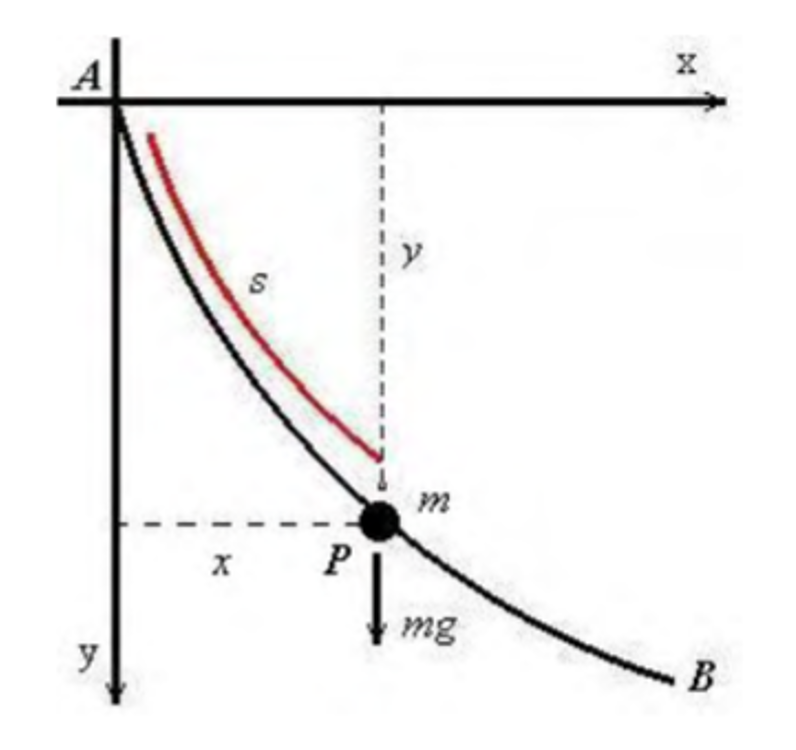
\includegraphics[scale=0.6]{imgs/braquistocrona.png}

  \end{figure}

Figura 4.1 - Esquema do Problema da Braquistócrona no Plano.

\end{center}

Por questões de conveniência o eixo $y$ está orientado no sentido oposto, dessa forma temos uma gravidade orientada no sentido positivo. Desenvolvendo os cálculos, vimos que a solução para esse problema é uma curva $y=y(x)$ que minimiza o funcional abaixo

\begin{center}
$J(y(\cdot)) = \dfrac{1}{\sqrt{2g}} \int_a^b \sqrt{\dfrac{1-y'^2}{y_0 - y}}\; \mathrm{d}x$,
\end{center}

onde g é a aceleração da gravidade e $y(a) = y_a$  o gráfico desta solução foi chamado de braquistócrona e é uma cicloide invertida.

\begin{itemize}
\item O Funcional
\end{itemize}

Em cada um dos problemas usados como motivação, sempre recaímos num funcional da forma

\begin{center}
$J(y(\cdot)) = \int_a^b f(x, y(x), y'(x)) \; \mathrm{d}x$,
\end{center}

sujeito a condições de fronteira $y(a) = y_a$, $y(b) = y_b$.
O propósito então é sempre maximizar ou minimizar o funcional cujo domínio é um espaço de funções, por exemplo, $C^1[a,b]$ espaço das funções $y:[a,b] \to \mathbb{R}$ continuas cuja primeira derivada é também contínua. Nesse espaço trabalhamos com dois tipos de normas:

\begin{itemize}
\item Norma Fraca
\end{itemize}

\begin{center}
$ ||h|| = m\acute{a}x|h(x)|, \; x \in [a,b] $
\end{center}

\begin{itemize}
\item Norma Forte
\end{itemize}

\begin{center}
$ ||h|| = m\acute{a}x|h(x)| + máx|h'(x)|, \;x \in [a,b] $
\end{center}

Partimos do princípio que o funcional possui um extremo $\hat{y}(x)$ e buscamos condições necessárias que ele deve satisfazer. Para isso tomamos uma pequena perturbação 
$y(x)= \hat{y}(x)+ \varepsilon\eta(x) de \hat{y}(x)$, onde $\eta(a)= \eta(b)=0$ e $\varepsilon>0$, de forma que 

\begin{center}
$J(\hat{y} + \varepsilon\eta) - J(\hat{y}) = \int_a^b f(x, \hat{y} + \varepsilon\eta, \hat{y}' + \varepsilon\eta') - f(x, \hat{y} + \varepsilon\eta, \hat{y}' + \varepsilon\eta') \; \mathrm{d}x $
\end{center}

Definimos a primeira e segunda variações por

\begin{center}

$\sigma J = \varepsilon \dfrac{dJ(\varepsilon)}{d\varepsilon}|_{\varepsilon=0}= \varepsilon \int_a^b [\dfrac{\partial f}{\partial y}(x, \hat{y}, \hat{y}')\eta + \dfrac{\partial f}{\partial y'}(x, \hat{y}, \hat{y}')\eta'] \; \mathrm{d}x $ (1)

$\sigma^2 J = \varepsilon^2 \dfrac{d^2 J(\varepsilon)}{d\varepsilon^2}|_{\varepsilon=0}= \varepsilon^2 \int_a^b [\dfrac{\partial^2 f}{\partial y^2}(x, \hat{y}, \hat{y}')\eta^2  + s \dfrac{\partial^2 f}{\partial y \partial y'}(x, \hat{y}, \hat{y}')\eta\eta'+ \dfrac{\partial^2 f}{\partial y'^2}(x, \hat{y}, \hat{y}')\eta'^2 ] \; \mathrm{d}x $ (2)

\end{center}

TEOREMA: Uma condição necessária para o funcional ter um mínimo local (ou máximo) em $\hat{y}(x)$ é que a primeira variação de $J(y(\cdot))$ seja nula, isto é $\sigma J=0$, para toda variação $\eta(x)$.

Usando integração por partes, reescrevemos $\sigma J=0$ na forma

\begin{center}
$\int_a^b \eta(x) [\dfrac{\partial f}{\partial y} - \dfrac{d}{dx}(\dfrac{\partial f}{\partial y'})] \; \mathrm{d}x = 0$
\end{center}

e como esta equação é válida para todo $\eta(x) \in C^1[a,b]$ tal que $\eta(a)=\eta(b)=0$ o Lema de Du Bois - Reymond nos diz que 

\begin{center}
$\dfrac{\partial f}{\partial y} - \dfrac{d}{dx}(\dfrac{\partial f}{\partial y'}) = 0 $ (3)
\end{center}

esta é a equação de Euler - Lagrange, ela nos diz que se $\hat{y}(x) \in C^2 [a,b]$ e é um extremo local de $J(y(\cdot))$, então $\hat{y}(x)$ deve satisfazer (3). Dessa forma, pelo uso das equações de Euler - Lagrange (3), encontramos que a curva que minimiza o funcional no problema da braquistócrona é a cicloide

\begin{center}
$x(\phi)= \alpha + R(\phi - \sin \phi) $\\
$y(\phi)= y_a  + R(1 - \cos \phi)$

\end{center}

Em seguida trabalhamos com funcionais que dependem de múltiplas funções, ou seja,

\begin{center}
$J(y_1, ... , y_n) = \int_a^b f(x,y_1, ... , y_n, y'_1, ... , y'_n) \; \mathrm{d}x$,
\end{center}

satisfazendo as condições de fronteira $y_i (a) = y_ia$, $y_i (b) = y_ib$, para $i=1,…,n$. Neste momento assumimos que as variáveis são independentes e a não existência de restrições. Agindo da mesma forma que anteriormente, buscamos condições necessárias que uma solução $\hat{y}(x)=(\hat{y}_1(x),...,\hat{y}_n(x))$ minimizadora deve satisfazer. Para isso, novamente, tomamos uma perturbação $y(x)= \hat{y}(x) + \varepsilon \eta(x)$, onde $\eta(x)=(\eta_i (x))$   e  $\eta_i (a)=\eta_i (b)  = 0$,
para $i =1,...,n$. Mais uma vez considerando a variação $J(\hat{y} + \varepsilon\eta) - J(\hat{y})$ como uma função de $\varepsilon$ e usando expansão de Taylor e Du Bois - Raymond, obtemos um sistema de equações de Euler - Lagrange

\begin{center}
$\dfrac{\partial f}{\partial y_i} - \dfrac{d}{dx}(\dfrac{\partial f}{\partial y_i'}) = 0 $, $ i = 1,...,n$ (4)
\end{center}

Para o caso particular, onde a variável independente $x$ não aparece explicitamente no Lagrangeano $f(y_1,...,y_n,y'_1,...,y'_n)$, o sistema (4) assume a forma

\begin{center}
$f - \sum_{i=1}^{n} \dfrac{\partial f}{\partial y'_i} y'_i = C$(5)
\end{center}

Os resultados obtidos são aplicados na mecânica - Lagrangeana, com o problema do pêndulo esférico. Nesse problema a variável independente $x$ denota o tempo $t$ e escrevemos $y(t)=q(t)=(q_1 (t),…,q_n (t))$, chamadas de coordenadas generalizadas. Tomamos o Lagrangeano como sendo

\begin{center}
$ f(t, q, \dot q) = K(t, q, \dot q) - U(t, q) $,
\end{center}

onde K é a energia cinética e U é a energia potencial e assumimos o princípio de Hamilton que nos diz que o movimento do sistema mecânico de $q(t_a)= q_a$  a  $q(t_b )= q_b$ é tal que a primeira variação da integral $S(q)= \int_{t_a}^{t_b}f(t,q,\dot q)\; \mathrm{d}t$ é zero.


\begin{itemize}
\item O Problema do pêndulo
\end{itemize}

No problema do pêndulo, esboçado abaixo, temos uma massa m no extremo de uma corda sem peso de comprimento l. Assim, o movimento da massa está restrito à esfera de raio l. Sendo $\theta$ o ângulo da corda com o eixo vertical e $\varphi$ o ângulo da projeção dessa corda com o eixo $x$.

\begin{figure}[!h]
    \centering
    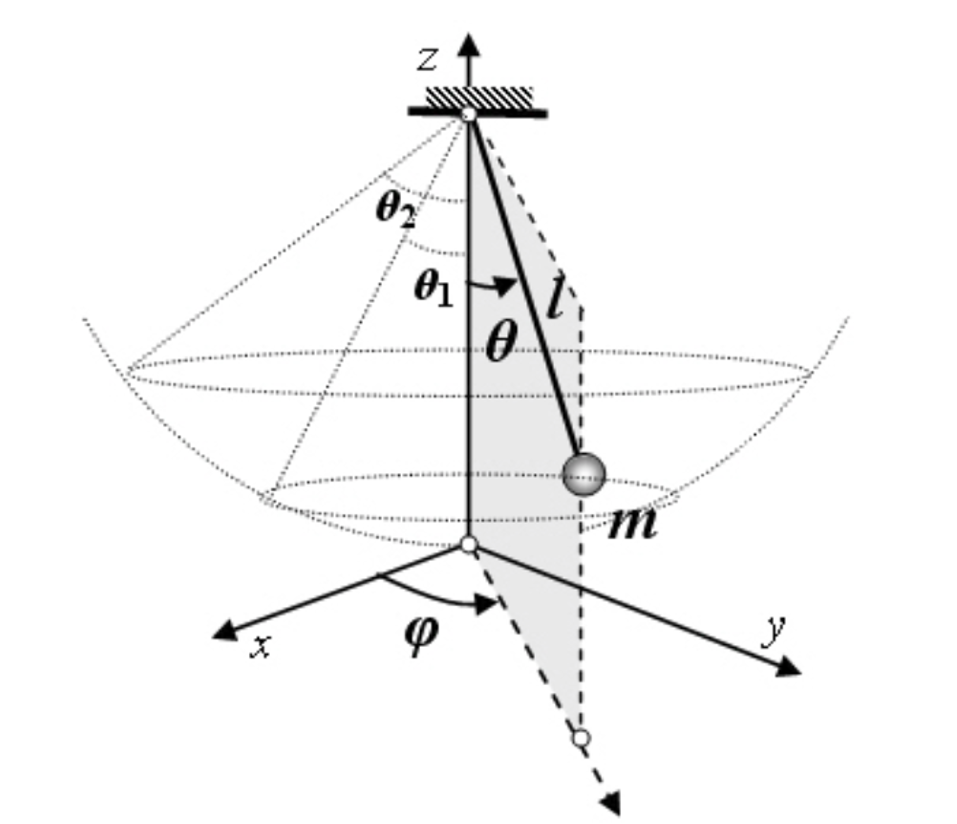
\includegraphics[scale=0.6]{imgs/pendulo.PNG}

  \end{figure}
  
\begin{center}
  Figura 4.2 - Esquema do Problema do pêndulo no Espaço.
  \end{center}  
  
Do modelo acima retiramos as seguintes expressões para as energias potencial e cinética, respectivamente,

\begin{center}
$U(\theta) = mgl(1-\cos\theta)$ e\\
$K(\theta, \varphi) = \dfrac{1}{2}ml^2({\dot \theta}^2 + {\dot \varphi}^2 \sin^2 \theta)$
\end{center}
  
Logo, o lagrangeano será

\begin{center}
$ f(\theta, \dot \theta, \dot \varphi) =  \dfrac{1}{2}ml^2({\dot \theta}^2 + {\dot \varphi}^2 \sin^2 \theta) - mgl(1-\cos\theta)$
\end{center}

Desde que f não dependa explicitamente de t, através da expressão (5) obtemos que

\begin{center}
$\dfrac{1}{2}ml^2({\dot \theta}^2 + {\dot \varphi}^2 \sin^2 \theta) - mgl(1-\cos\theta) = E$,
\end{center}

onde E é a energia total do sistema. Logo a função $q(t)=(\theta(t),\varphi(t))$ que minimiza o potencial para o movimento, deve satisfazer esta equação.

Continuando com o estudo, relacionamos o Lagrangeano ao Hamiltoniano, buscando reescrever o sistema das n equações (4) como um sistema de 2n equações diferenciais de primeira ordem.
Seja $F: \mathbb{R} \to \mathbb{R}^3$ uma função que para cada tempo t associa uma força $F(t)=(f_1(t),f_2(t),f_3(t))$ num espaço de configurações $q(t)=(q_1(t),q_2(t),q_3(t))$. Da Segunda Lei de Newton $F(t)=m\ddot q(t)=  \dfrac{d}{dt}(mq(t))$, considerando $F(t)$ um campo conservativo, temos que

\begin{center}
$ F(t) = -grad U(t, q(t)) $ (6),
\end{center}

onde $P(t) = U(t,q(t))$ é a energia potencial. Fazendo $K(t)= \dfrac{1}{2} m||\dot{q}(t)||^2$ a energia cinética, segue que a energia total é dada por $H(t)=P(t)+K(t)$.
Vimos anteriormente que 

\begin{center}
$ f(t, q(t), \dot{q}(t)) = \dfrac{1}{2} m||\dot{q}||^2 -U(t, q(t)) $ (7)
\end{center}

Além disso, o Princípio da Menor Ação de Hamilton nos diz que se $\hat{q}(t)$ é um mínimo do funcional $J(q(t))= \int_{t_0}^t f(s,q(s),\hat{\dot{q}}(s)) \; \mathrm{d}s$, então 

\begin{center}
$ \dfrac{\partial f}{\partial q_i}(t, \hat{q}(t), \hat{\dot{q}}(t)) - \dfrac{d}{dt} \dfrac{\partial f}{\partial q_i}(t, \hat{q}(t), \hat{\dot{q}}(t)) = 0$ , para $i = 1,2,3$ (8).
\end{center}

Assim, 
\begin{center}
$H(t) = \dfrac{1}{2} m \sum_{i=1}^{3} [\dot{q}(t)]^2 + U(t,q(t))$\\
$H(t) = -\dfrac{1}{2} m \sum_{i=1}^{3} [\dot{q}(t)]^2 + m \sum_{i=1}^{3} [\dot{q}(t)]^2 + U(t,q(t))$\\
$H(t) = -K(t) + P(t) + \sum_{i=1}^{3} \dot{q_i}(t)[m\dot{q}_i(t)]^2 $\\
$H(t) = -f(t, q(t), \dot{q}(t)) + \langle \dot{q}(t), p(t) \rangle$ (9)
\end{center}

onde $p(t) = mq(t)$ é o momento. Note que para cada $j = 1,2,3$, $p_j=  \frac{\partial f}{\partial \dot{q}_j}$. A expressão (9) é chamada de transformada de Legendre. Podemos, portanto, reescrever (8) na forma

\begin{center}
$\dfrac{d}{dt}(m\dot{q}_i(t)) = \dfrac{\partial f}{\partial \dot{q}_i}(t, q(t), \dot{q}(t))$
\end{center}

e através de (9), obtemos o sistema Hamiltoniano com $2n$ equações de Primeira Ordem

\begin{center}
$\dot{p}_i(t)= -\dfrac{\partial H}{\partial q_i} $
$\dot{q}_i(t)=  \dfrac{\partial H}{\partial p_i} $

\end{center}


A etapa seguinte consistiu em estudar extremos do funcional $J(y(\cdot))$ com restrições. Foram trabalhados três tipos de restrições: Isoperimétricas, Holonômicas e Não - Holonômicas. A primeira na forma de condições integrais

\begin{center}
$k(y) = \int_a^b g(x, y, y') \; du = 1$,
\end{center}

como no problema da rainha Dido; e as outras duas diferenciando-se conforme envolva as derivadas y' ou não: 

\begin{center}
$g(x,y_1,...,y_n) = 0 $ (Holonômicas)\\
$g(x,y_1,...,y_n, y'_1,...,y'_n) = 0 $ (Não Holonômicas)
\end{center}

Exemplificamos apenas os dois primeiros tipos.

Para manipular essas restrições usamos multiplicadores de Lagrange. Por exemplo, no caso isoperimétrico, considerando uma perturbação do tipo $y(x)=y(x)+ \varepsilon_1 \eta_1 (x)+ \varepsilon_2 \eta_2 (x)$, com $\eta_1(a)=\eta_2(a) = 0$ e $\eta_1(b)=\eta_2(b)= 0$, concluímos que primeiro devemos encontrar extremos para o funcional $\int_a^b[f(x,y,y') - \lambda g(x,y,y')]\; dx$, para $\lambda$ constante, na forma $y=y(x,\lambda,c_1,c_2)$, onde $c_1$  e  $c_2$ são constantes a serem determinadas através das condições de fronteira. Na sequência, usamos a segunda variação (2) para retirar condições sobre um extremo do funcional $J(y)$ sujeito às condições de fronteira $y(a)= y_a$ e $ y(b) = y_b$. Desde que $\delta J=0$, segue da expansão $\Delta J= \delta J+\dfrac{1}{2} \delta^2 J+O(\varepsilon^3)$ que para $\varepsilon$ suficientemente pequeno a variação total é dominada por $\delta^2 J$. Assim para que o funcional tenha um mínimo local em $\hat{y}(x) \in C^1 [a,b]$, é necessário que $\delta^2 J \ge 0$, para todo $\eta(x) \in C^1 [a,b]$ que se anula em a e b.

\begin{itemize}
\item Condição de Legendre
\end{itemize}

Buscando uma condição sobre variações fortes, estudamos a condição de Legendre que afirma que uma condição necessária para o funcional $J(y)$ ter um mínimo local em $\hat{y}(x)$ é que 

\begin{center}
$R(x) = \dfrac{\partial^2 f}{\partial y'^2}(x,\hat{y}(x),\hat{y}'(x)) \ge 0$ em  $[a,b]$
\end{center}

Encerramos o estudo de Cálculo variacional investigando condições para um extremo local forte $\hat{y}$ do funcional $J(y)$. Nesse caso, podemos considerar $\hat{y}$ uma função contínua por partes no intervalo [a, b]. Supondo a existência de um ponto de canto $c \in [a,b]$, tomamos duas perturbações $\eta_1$ e $\eta_2$ agindo sobre as duas porções de $\hat{y}$ (antes e depois de c):

\begin{center}
$y_1(x)=\hat{y}(x)+ \varepsilon \eta_1(x)$, $\eta_1(a)=0$ e\\
$y_2(x)=\hat{y}(x)+ \varepsilon \eta_2(x)$, $\eta_2(a)=0$.
\end{center}

Dessa forma, o funcional J é escrito como uma soma de dois funcionais, onde cada uma das funções de $\hat{y}$ deve ser um extremo do funcional correspondente $J_i$. Considerando a primeira variação $\delta J_1=0$ e $\delta J_2=0$, obtemos a condição de Weierstrass-Erdmann que nos diz que se $\hat{y}$ é um extremo forte de $J(y(\cdot))$ então  $\dfrac{\partial f}{\partial y'}$ e $y'\dfrac{\partial f}{\partial y'}-f$ devem ser contínuos em cada lado do canto c.

Para um determinado Lagrangeano f(x,y,z), a função excesso de Weierstrass é definida por 

\begin{center}
$E(x,y,z,y) = f(x,y,w) - [f(x,y,z) + (w-z)f_3 (x,y,z)]$ (10),
\end{center}

que pode ser pensada como a primeira aproximação de Taylor para f(x,y,w) em torno de z. Assim, de modo equivalente obtemos que se $\hat{y}$ é um mínimo forte de J, então $E(x,\hat{y}(x),\hat{y}'(x), w) \ge 0$,   para todo $w \in \mathbb{R}$ e todo $x \in [a,b]$ que não são cantos.

Da transformada de Legendre, $H(x,y,z,p)=pz-f(x,y,z)$ e da equação (10), encontramos que 

\begin{center}
$E(x,y,z,w)=H(x,y,z,p)-H(x,y,w,p)$,
\end{center}

de modo que, se $\hat{y}$ é um mínimo forte local para J, então $\hat{y}$ maximiza o Hamiltoniano H(x,y,w,p), para todo $x \in [a,b]$. Este é o princípio do máximo de Weierstrass.

\begin{itemize}
\item Controle Ótimo Linear Feedback
\end{itemize}

Em seguida foi introduzido o Regulador Linear Quadrático. Dado Um sistema descrito por um conjunto de equações diferenciais lineares e um custo descrito por uma função quadrática, o Regulador LQ provê a solução do problema Linear Quadrático.
Seja $\dot{x} = f(x,u) = A(t)x + B(t)u$, sendo $x(t_0) = x_0$, com $x \in \mathbb{R}^n, u \in \mathbb{R}^m$  e o conjunto alvo sendo $S= \lbrace t_1\rbrace \times \mathbb{R}$ (Horizonte Finito) o funcional a ser minimizado é

\begin{center}
$ J(u) = \int_{t_0}^{t_1} (x^tQ(t)x + u^tR(t)u) \; dt + x^t(t_1)Mx(t_1) $
\end{center} 

Segundo a transformada de legendre, podemos escrever a Hamiltoniana  da seguinte forma

\begin{center}

$H(x,u) = -p_0L(x,u) + \langle p, f(x,u) \rangle$, $p_o = 1$ \\
$H(x,u) = -x^tQ(t)x - u^tR(t)u + \langle p, A(t)x + B(t)u \rangle$\\
$H(x,u) = -x^tQ(t)x - u^tR(t)u + \langle p, A(t)x \rangle + \langle p, B(t)u \rangle$\\\

$ \dfrac{\partial H}{\partial u} = 0 $\\
$ B^tp - 2R(t)u^* = 0 $\\
$u^* = \dfrac{1}{2}R^{-1}B^tp(t)$\\
\end{center}

onde $u^*$ ... e $p(t)$ é a solução da equação de Riccati 

\begin{center}
$ \dot{p}(t) = -p(t)A(t) - A^t(t)p(t) - Q(t) + p(t)B(t)R^{-1}(t)B^t(t)p(t)$
\end{center}
\newpage

\section{Metodologia}

A pesquisa é classificada, tanto do ponto de vista dos procedimentos metodológicos, quanto da natureza, como uma pesquisa bibliográfica, uma vez que os estudos foram feitos a partir de materiais já publicados. Periodicamente, houve encontros entre orientando e orientador para discussão e exposição do conteúdo estudado. Ao final, para colocar em prática os conteúdos apresentados, foi proposta a implementação de código computacional para reproduzir as simulações obtidas em um dos trabalhos, usados como fonte de estudo.
\cite{Burns2014}
\newpage

\section{Resultados e discussões }
\section{Conclusões}
\section{Perspectivas}

\newpage

\section{Referências bibliográficas}
\bibliography{pibic-2018.bib}
	
\newpage

\section{Outras atividades}
Além dos encontros em sala para apresentação do conteúdo introdutório ao assunto,
participei, como atividade complementar, do 27º Encontro de Iniciação Científica da UFS.
Minicurso sobre GERENCIAMENTO DE REFERÊNCIAS BIBLIOGRÁFICAS PARA
TRABALHOS DE PESQUISA E ARTIGOS CIENTÍFICOS. No dia 21/11/2017. E do II SSMAC 2018 (Série de Seminários de Matemática Aplicada e Computacional). Palestra sobre UM MODELO PARA CONSTRUIR FOTOGRAFIAS PANORÂMICAS. Dia 20/04/2018.\

\end{document}
